% !TeX spellcheck = en_GB
% !TeX encoding = UTF-8
% !TeX root = ../report.tex

\chapter{Results and Discussion}
\label{chp:Results}

\section{Testing}


\subsection{Linear motor}

To find the optimal parameters of the linear motor, we used a simple spring setup and the LinMot Talk software. With the software, we were able to adjust any motor parameters in real-time, have it perform different moves at various speeds and accelerations. \\On the spring gauge, which was clamped in between the linear motor and the beam, we could read off the force and compare it to the calculated force in LinMot Talk. We found out that the maximum stroke was mostly limited by the maximum velocity. The maximum required stroke of around 55 mm can be reached with a maximum velocity of around 1.5 m/s and maximum acceleration.
 
A maximum velocity higher than that leads to the motor shutting down, which is something we certainly wanted to avoid. 
  
The temperature of the drive rises to critically high temperatures only after maintaining a considerably high force of above 200 N. Since such a force is only required for a very hard brake it should be possible to prevent longer periods of braking with more than 200 N. The following graphs show the winding-temperature change of the motor for different forces exerted on the drive.
% Graphiken
Note that the drive overheats in the emergency brake simulation only after x seconds which is much longer than the average duration of an emergency brake.

\begin{figure}[h]
	\centering
	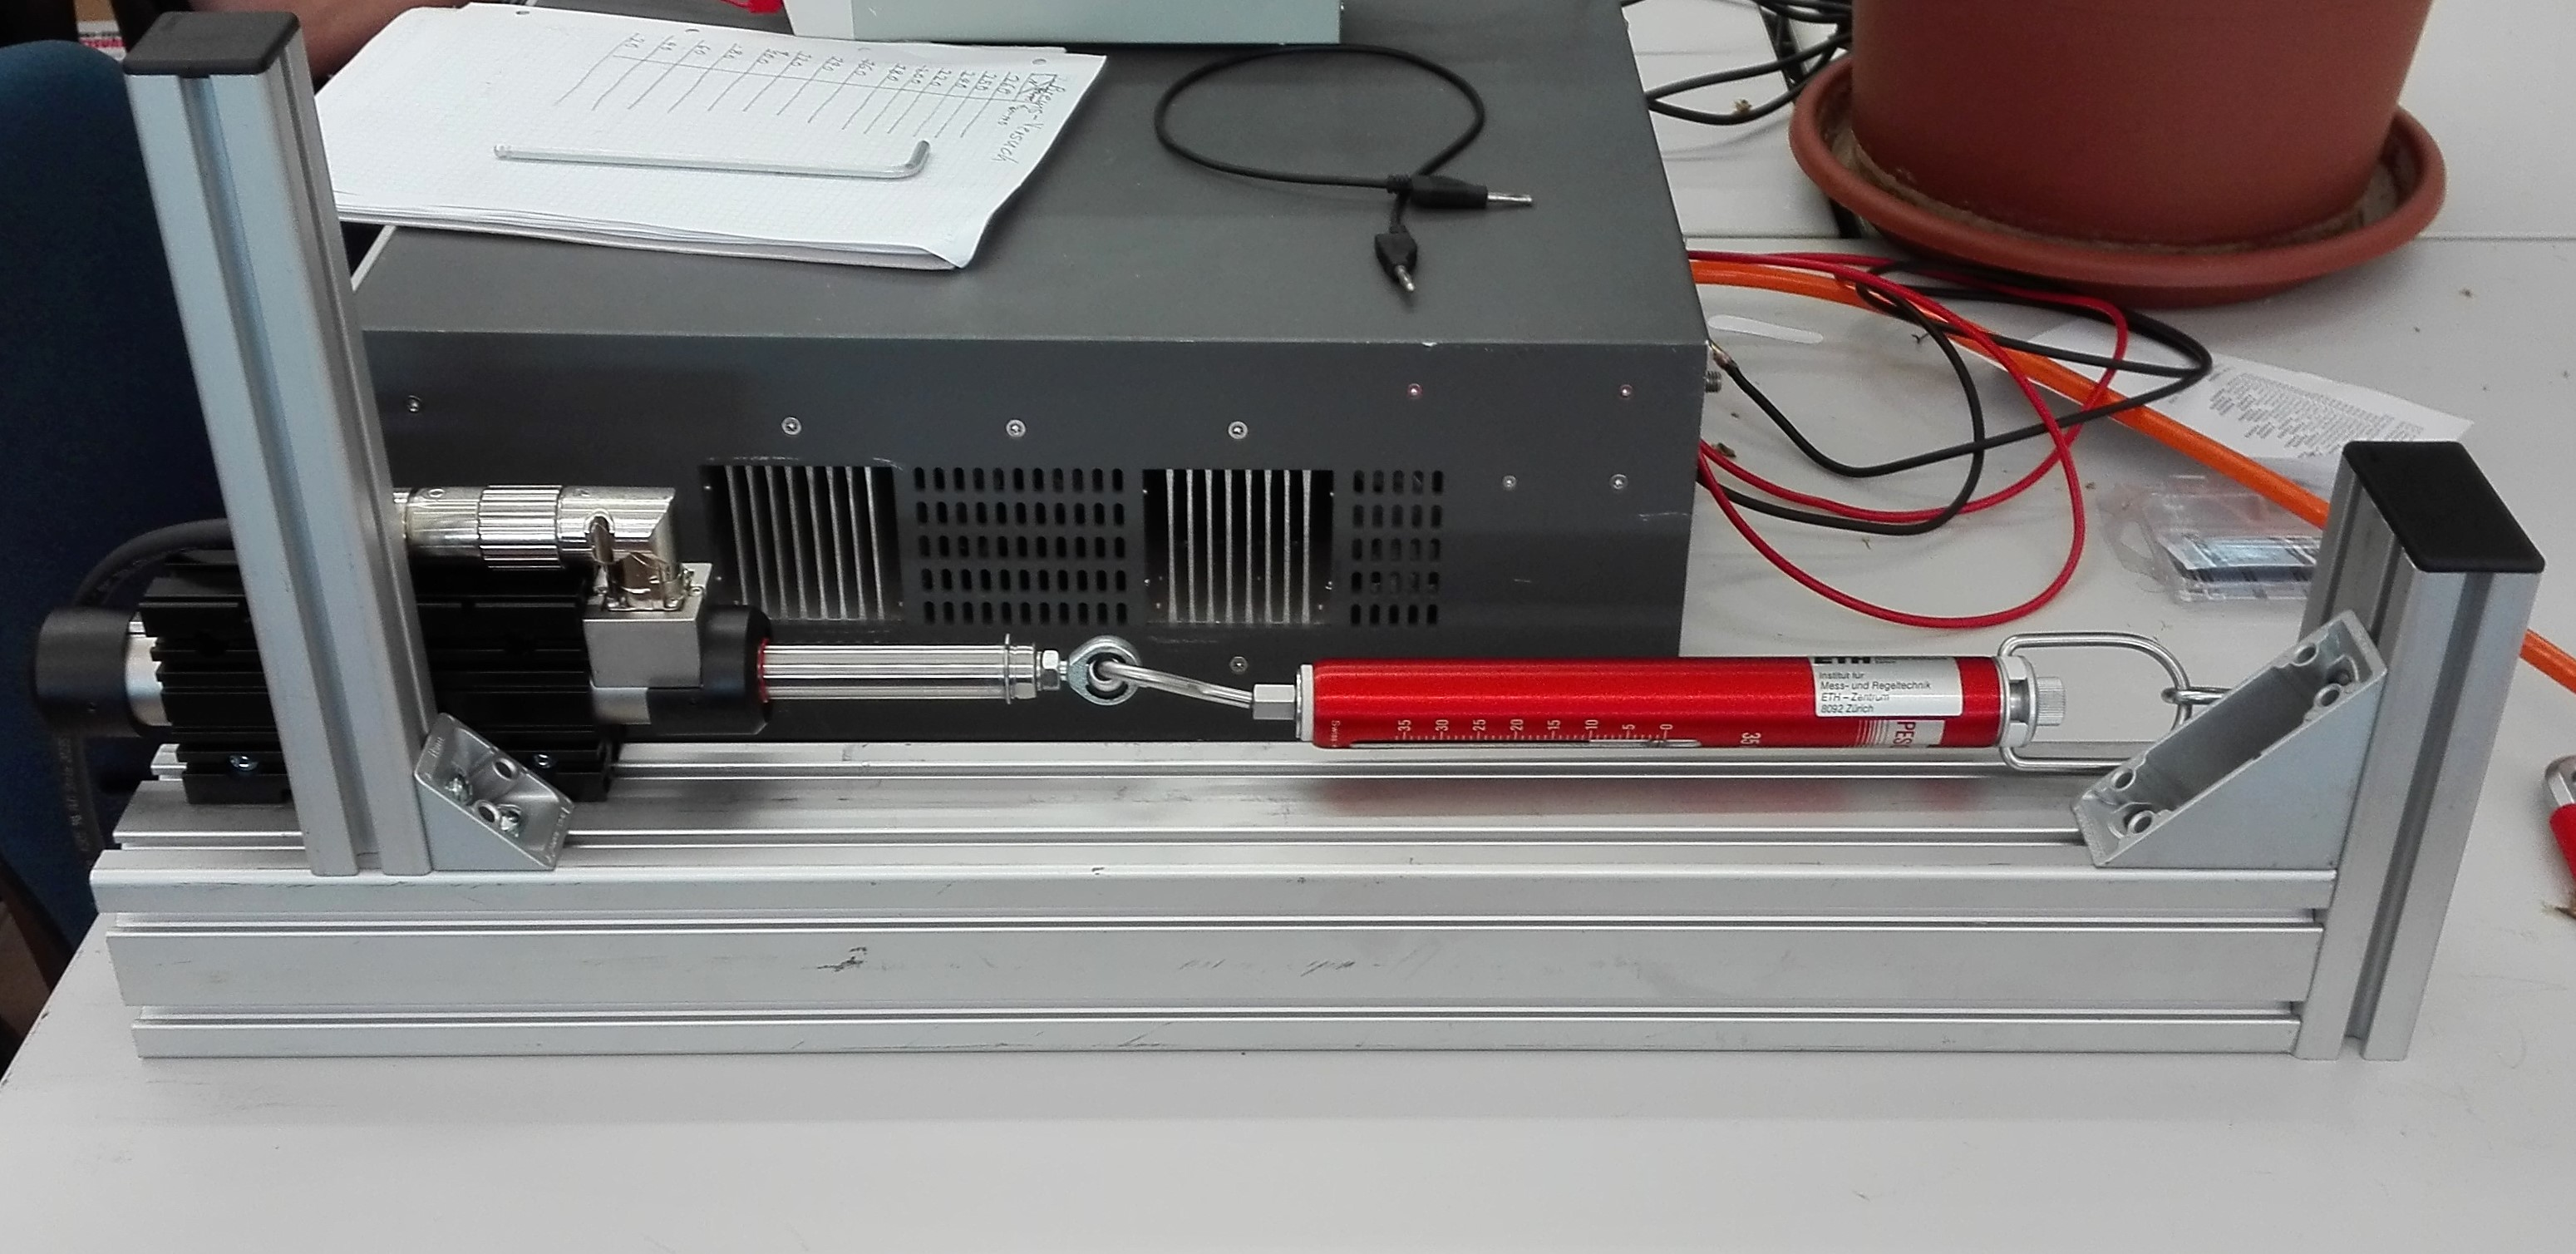
\includegraphics[width=0.7\linewidth]{pictures_figures/Used/Picture_linmottest}
	\caption{}
	\label{fig:picturelinmottest}
\end{figure}



\subsection{Brake}
A first proof of concept for the brake was made with the brake mounted on the kart and a driver actuating the brake maneuver with a button.
The brake was supplied with power from the kart battery.


For this test, the analog inputs of the Linmot motor driver were used to trigger a brake maneuver previously setup on the Linmot driver. A range of braking curves were tested, from a slight brake to an emergency brake. The speed of the kart during the brakes was around 50 km/h.

In a first test without actuating the brakes at all it was noted that the kart stops considerably fast only with regenerative braking and friction acting on the kart.
The first, shorter braking strokes resulted in almost negligible difference to the test without braking.
However, the emergency brake resulted in locked wheels.

This proofed that a maximal braking force could be achieved and showed that the linear motor can be used while on the kart. The test was performed without external power supplies and the only input into the Linmot driver being the analog input from the braking button. During the test while trying to execute an emergency brake, one of the fuses blew. The fuses in the kart were rated up to 10 A while the linear motor's peak current however is around 25 A. The fuse was subsequently replaced with a suitable new one. 
 
It shall be noted that this test was performed with a driver in the kart at all time while the final kart will be driving without passenger and therefore be significantly lighter. This leads to a reduced requirement of force for an emergency brake because locking of the wheels will take place earlier.
%The precision of the linear motor was not yet determined fully, which would follow in subsequent tests.

In subsequent test we plotted the motors actual position, force and winding temperature with LinMot Talk's oscilloscope function. The test was done once for a hard brake and once for a soft brake. It is important to note that all data is merely calculated by the LinMot software, and thus does not reflect the actual values perfectly. However it is precise enough to analyse the motor's performance.

%\begin{figure}[h]
%	\centering
%	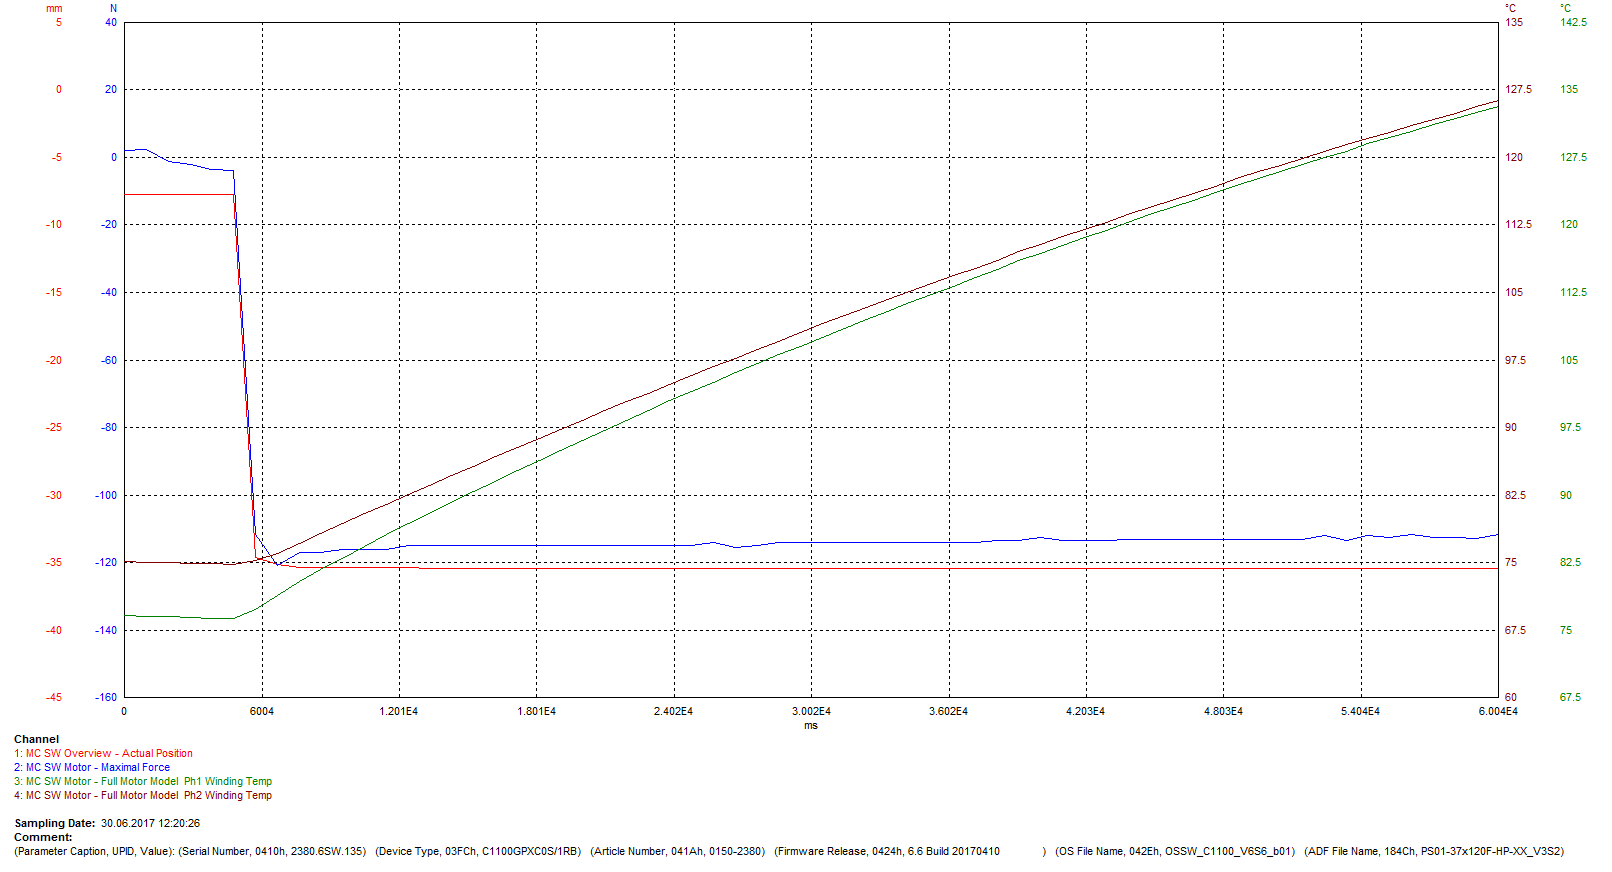
\includegraphics[width=1\linewidth]{pictures_figures/oscilloscope_neg36}
%	\caption{}
%	\label{fig:oscilloscopeneg36_rot}
%\end{figure}

\begin{figure}
	\centering
	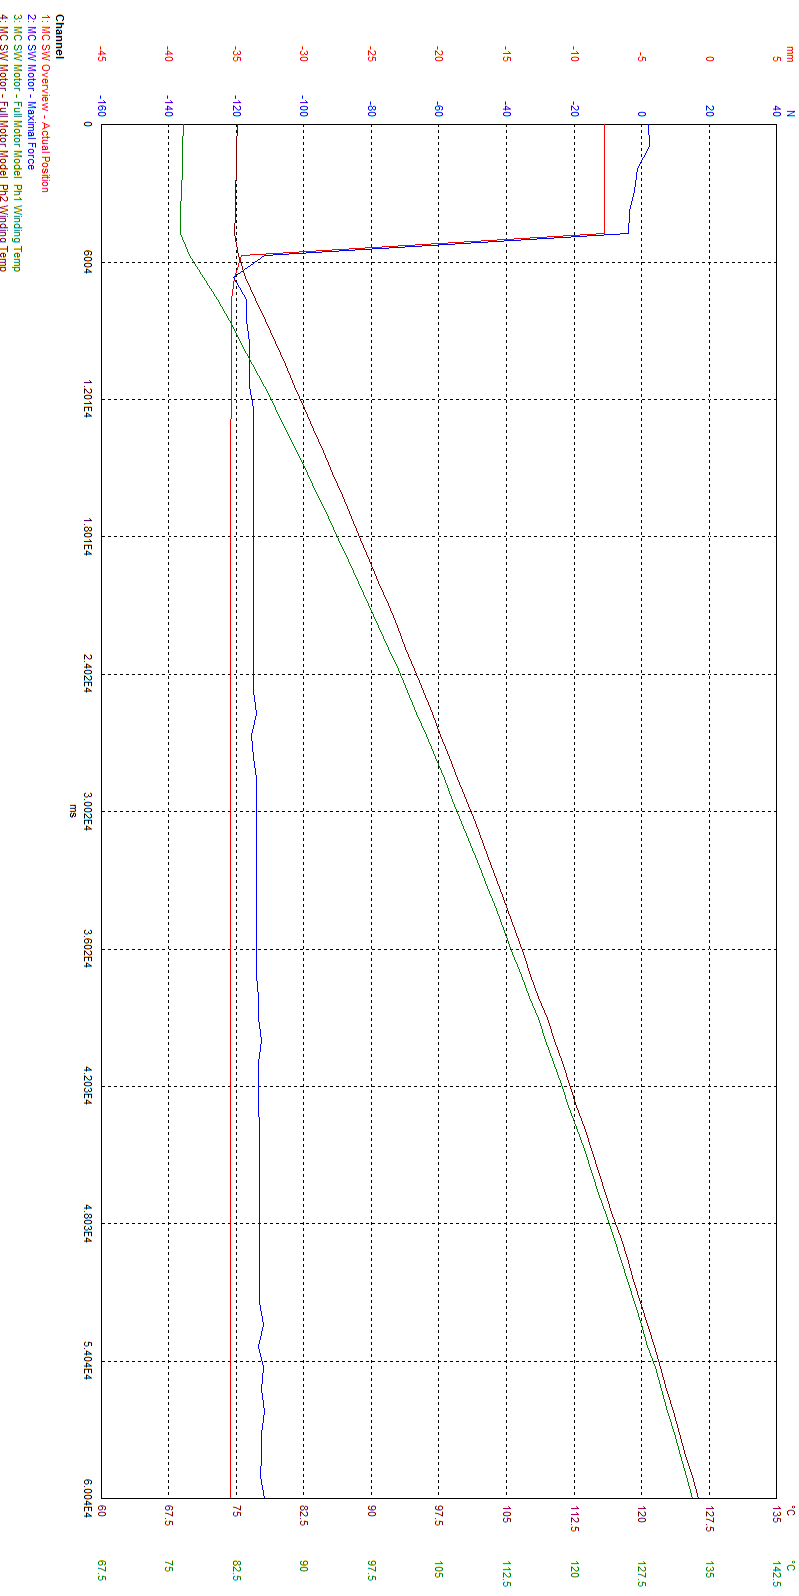
\includegraphics[width=0.7\linewidth]{pictures_figures/oscilloscope_neg36_rot}
	\caption{}
	\label{fig:oscilloscopeneg36rot}
\end{figure}


In \cref{fig:oscilloscopeneg36_rot} the oscilloscope recorded 60 seconds of data. This test was done to have a better understanding of how the motor overheats. At around 6 seconds, the motor reaches its demand position of -36 mm. At around the same time, the two windings of the motor start to heat up. The curve can more or less be assumed to be linear. Even after 54 seconds of operational time, the motor does not overheat and winding one still has around 15 °C left until it reaches its error temperature of 150°C. 

\begin{figure}
	\centering
	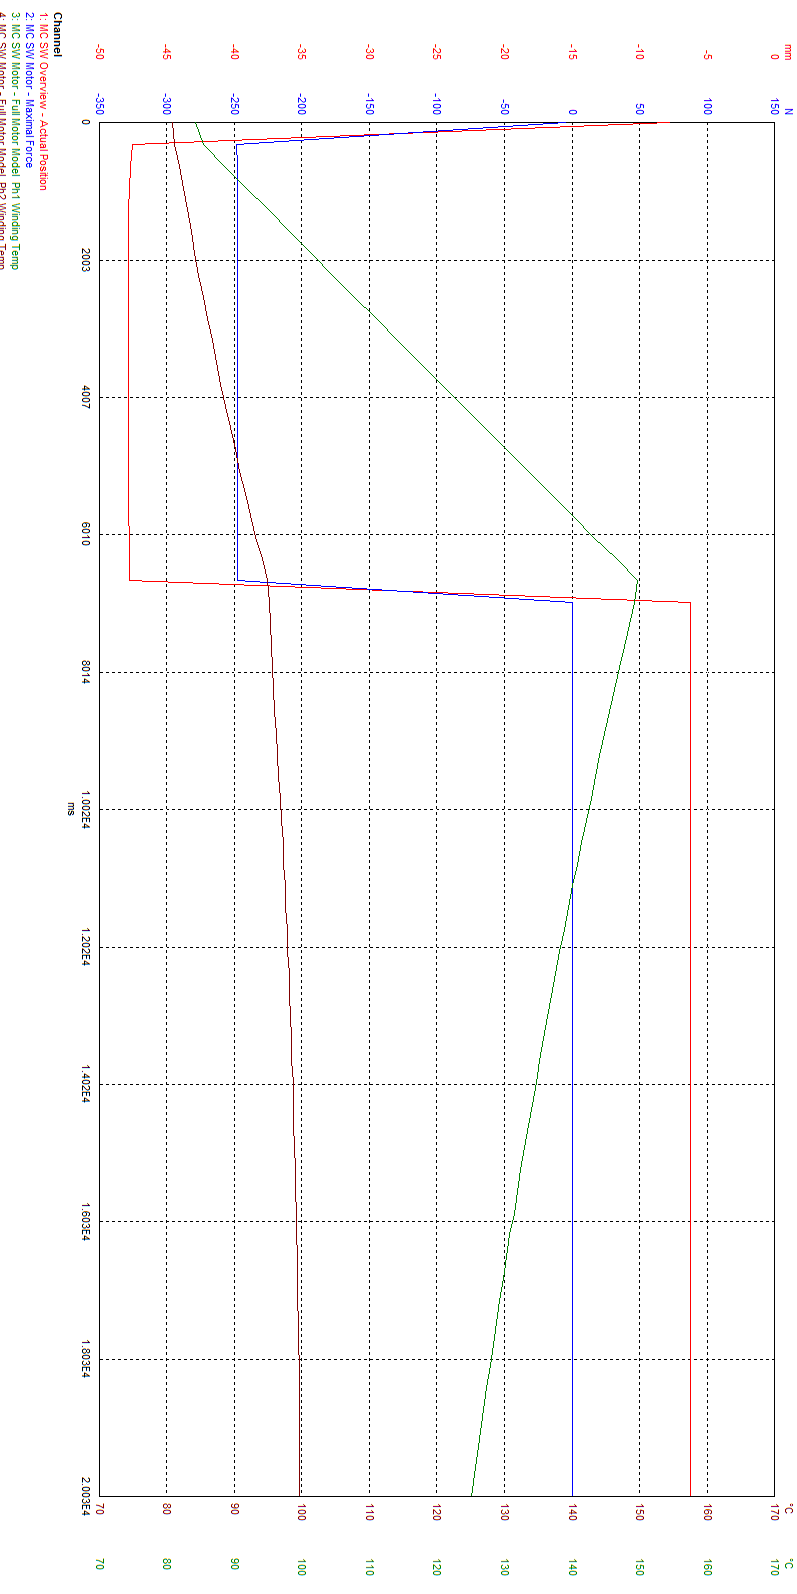
\includegraphics[width=0.7\linewidth]{pictures_figures/oscilloscope_neg54_rot}
	\caption{}
	\label{fig:oscilloscopeneg54rot}
\end{figure}

%\begin{figure}[h]
%	\centering
%	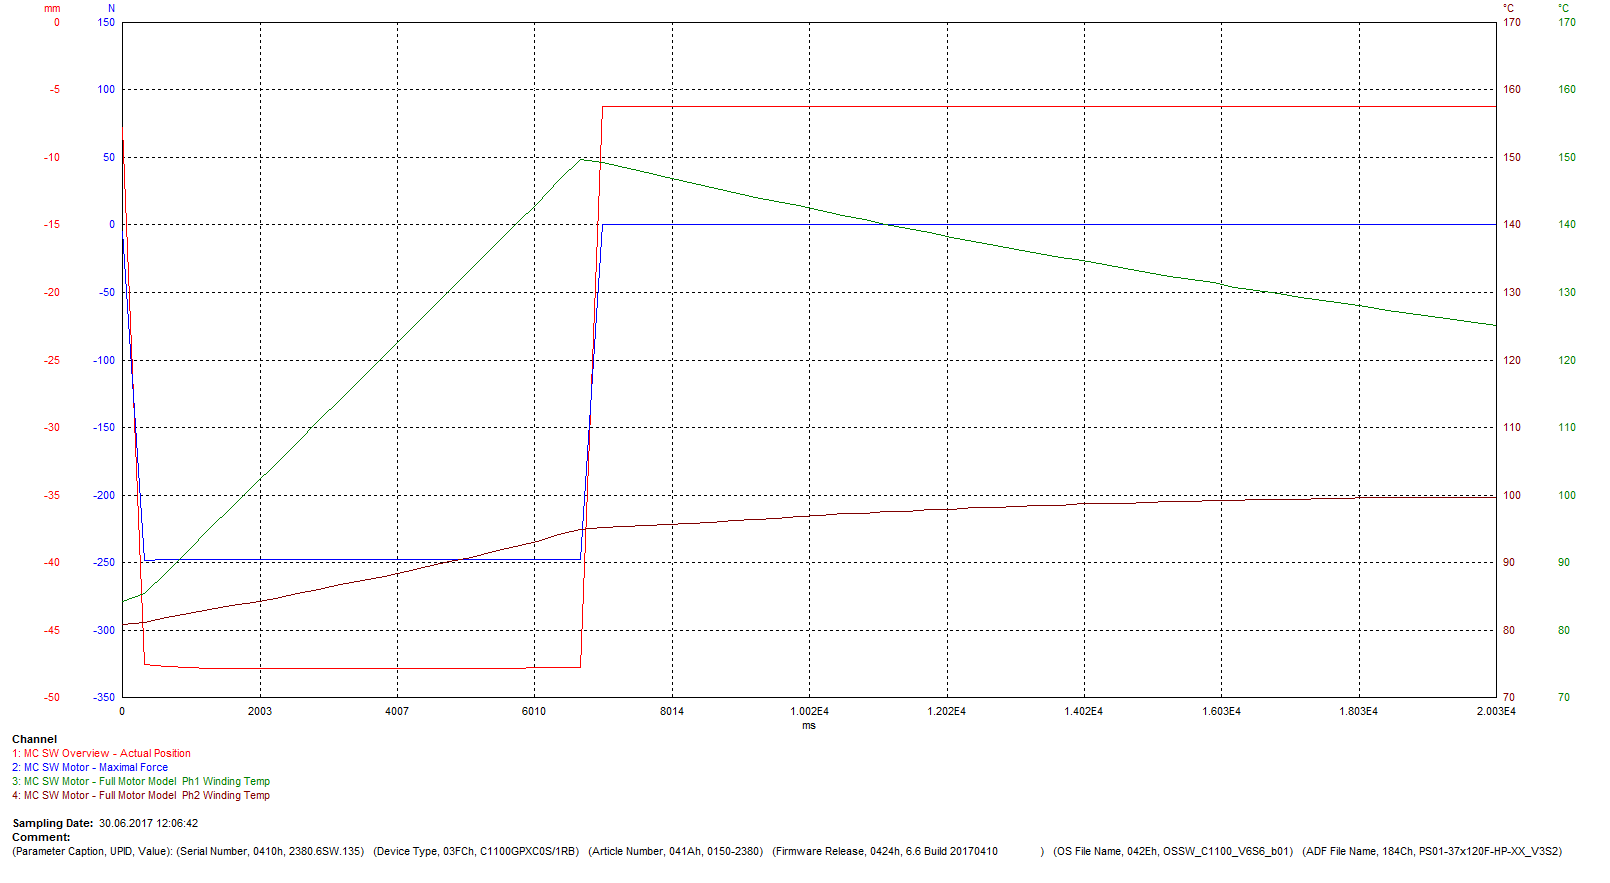
\includegraphics[width=1\linewidth]{pictures_figures/oscilloscope_neg54}
%	\caption{}
%	\label{fig:oscilloscopeneg54_rot}
%\end{figure}

In \cref{fig:oscilloscopeneg54_rot} the oscilloscope was used to record when the motor overheats for a hard brake and how exactly it reacts. For this a demand position of -54 mm was given, however the position will not be reached even with an integrator. This is because the motor's maximum force of around 248 N is reached and the slider can not extend any further. In this plot it is apparent that winding one overheats much quicker than winding two. As soon as 150°C is reached, the motor shuts down and the actual position, as well as the force return to zero. In this state the motor is in an error state and no further commands can be executed. The error needs to be acknowledged and the switch on bit has to be reset. After this procedure, the motor is back in the operational state.

\newpage

\subsection{Throttle}

To confirm the throttle's functionality, we plotted the kart's wheels actual speed, which is transmitted in PDO1(tx). 
